\documentclass{article}
\author{}

\usepackage{graphicx}
\usepackage{wrapfig}
\usepackage{enumerate}
\usepackage{hyperref}
\usepackage{float}
\usepackage[margin = 2.25cm]{geometry}
\usepackage[table]{xcolor}
\usepackage{fancyhdr}
\hypersetup{
  colorlinks = true,
  urlcolor = blue
}
\setlength\parindent{0pt}
\pagestyle{fancy}
\fancyhf{}
\rhead{College of Engineering, Construction and Living Sciences\\Bachelor of Information Technology}
\lfoot{Practical 08 Django 2: View \& Template \\Version 2, 2021}
\rfoot{\thepage}

\begin{document}

\begin{figure}
	\centering
	
\includegraphics[width=50mm]{./img/logo.png}
\end{figure}

\title{College of Engineering, Construction and Living Sciences\\Bachelor of Information Technology\\IN608: Intermediate Application Development Concepts\\Level 6, Credits 15\\\textbf{Practical 08 Django 2: View \& Template}} 
\date{}
\maketitle

\textbf{Due Date:} 07-05-2021 at 5pm \\

In this practical, you will complete a series of tasks covering today's lecture. This practical is worth 1\% of the final mark for the IN608: Intermediate Application Development Concepts course. \\

Before you start, in your practicals repository, create a new branch called \textbf{08-practical}.

\section*{Task 1} 
Create a Django project called \texttt{quiz}. \texttt{cd} to \texttt{quiz}, create a virtual environment \& install Django. Create an app called \texttt{practical08quiz}. Please ensure you configure your app in \texttt{quiz/settings.py} \& \texttt{quiz/urls.py}. \texttt{cd} to the \texttt{practical08quiz} directory \& create a Python file called \texttt{urls.py}. In \texttt{urls.py}, set the \texttt{app\_name} to \texttt{practical08quiz} \& create a URL which maps to the \texttt{index} function in \texttt{views.py}. In the \texttt{practical08quiz} directory, create a directory called \texttt{templates} \& sub-directory called \texttt{practical08quiz}. In \texttt{templates/practical08quiz}, create an \texttt{HTML} file called \texttt{index.html}. \\

In \texttt{views.py}, create a function called \texttt{index}. In this function, you will make a \texttt{GET} request to the \texttt{OpenTDB API} using the \texttt{Requests} Python module. \textbf{Note:} You will need to install \texttt{Requests} Python module in your virtual environment. Please ensure correct error checking, for example, not being able to make a \texttt{GET} request to the \texttt{OpenTDB API}. In this instance, you would raise a \texttt{ConnectionError} using the \texttt{Requests Exceptions} interface. Create a dictionary called \texttt{context}. This will be a dictionary of values (either the response contents from the \texttt{GET} request or an error message) to add to the template context. \\ 

The response contents should be in a \texttt{JSON (JavaScript Object Notation)} format. For example, if I make a \texttt{GET} request to \href{https://opentdb.com/api.php?amount=5\&type=multiple}{https://opentdb.com/api.php?amount=5\&type=multiple}, the response contents would look like the following: \\

\begin{figure}[H]
	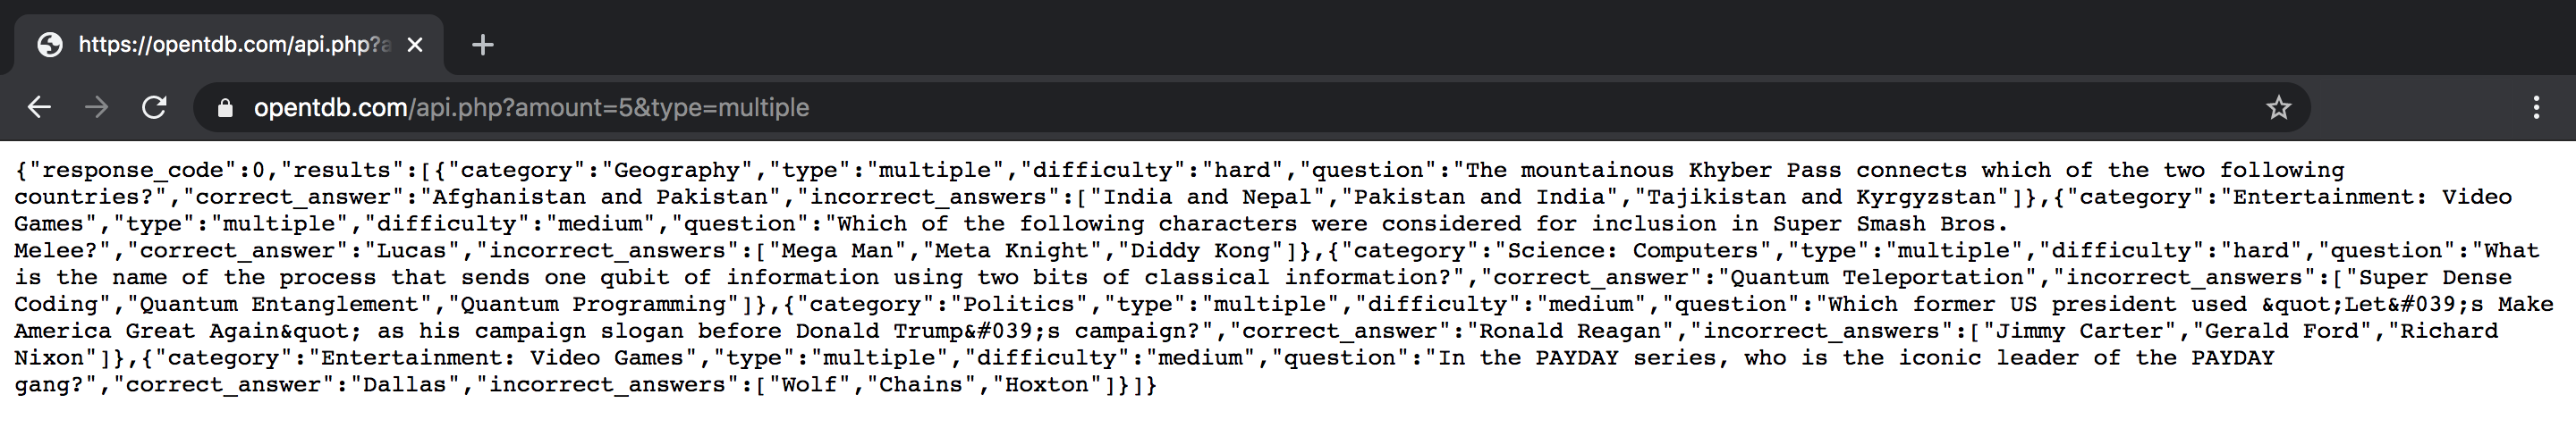
\includegraphics[width=175mm, height=35mm]{./img/08-quiz-json.png}
\end{figure}

\textbf{Note:} If the page is reloaded, the response contents will be different. \\

Pay careful attention to the \texttt{response\_code} key in the response content. This is appended to each API call to help tell developers what the API is doing. Below is a description of each \texttt{response\_code}:
\begin{itemize}
  \item \texttt{response\_code:} \texttt{0} or \texttt{Success} - returned results successfully.
  \item \texttt{response\_code:} \texttt{1} or \texttt{No results} - could not return results. The API does not have enough questions for your query.
  \item \texttt{response\_code:} \texttt{2} or \texttt{Invalid parameter} - contains an invalid parameter. Parameters passed in are not valid, i.e, \href{https://opentdb.com/api.php?amount=five}{https://opentdb.com/api.php?amount=five} 
  \item \texttt{response\_code:} \texttt{3} or \texttt{Token not found} - session token does not exist.
  \item \texttt{response\_code:} \texttt{4} or \texttt{Token empty} - session token has returned all possible questions for the specified query. Resetting the token is necessary.
\end{itemize}

Please ensure you check for all response codes. If \texttt{response\_code} is 1-4, add an error message to the \texttt{context} dictionary. \\ 

In \texttt{index.html}, display \texttt{context} in a nicely formatted \texttt{HTML} table. Use the \texttt{capfirst} filter to capitalise the first letter of each \texttt{difficulty} value. You may notice that some questions \& answers contain character entities, i.e., \texttt{\&quot;}. Use the \texttt{safe} filter to mark a value as not requiring further \texttt{HTML} escaping before outputting. For example, the \texttt{question} value \texttt{Who is the founder of \&quot;The Lego Group\&quot;?} would be marked as not requiring further \texttt{HTML} escaping. Instead, the output would be \texttt{Who is the founder of "The Lego Group"?} \& not contain \texttt{quot;} or other character entities. \\

Next week, we will look at how to serve static files, i.e., \texttt{CSS}, \texttt{JavaScript}, images, etc. Until then, internal styling will be accepted. 

\subsection*{Expected Output} 
Run the command \texttt{python manage.py runserver} then navigate to \href{http://127.0.0.1:8000/practical08quiz/}{http://127.0.0.1:8000/practical08quiz/} \\

\textbf{Note:} The incorrect answers column span is 3.

\begin{figure}[H]
  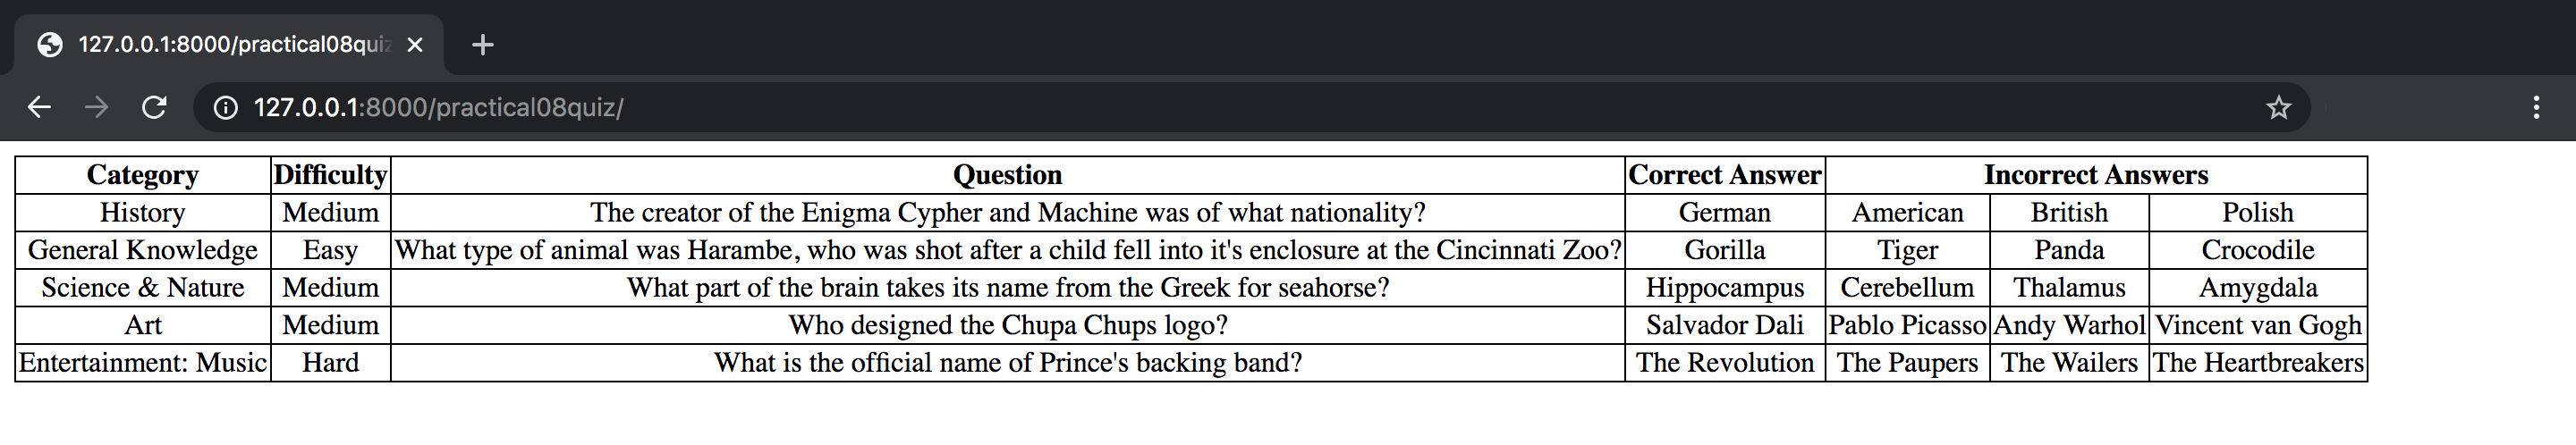
\includegraphics[width=175mm, height=35mm]{./img/08-expected-quiz-1.png}
\end{figure}

\begin{figure}[H]
  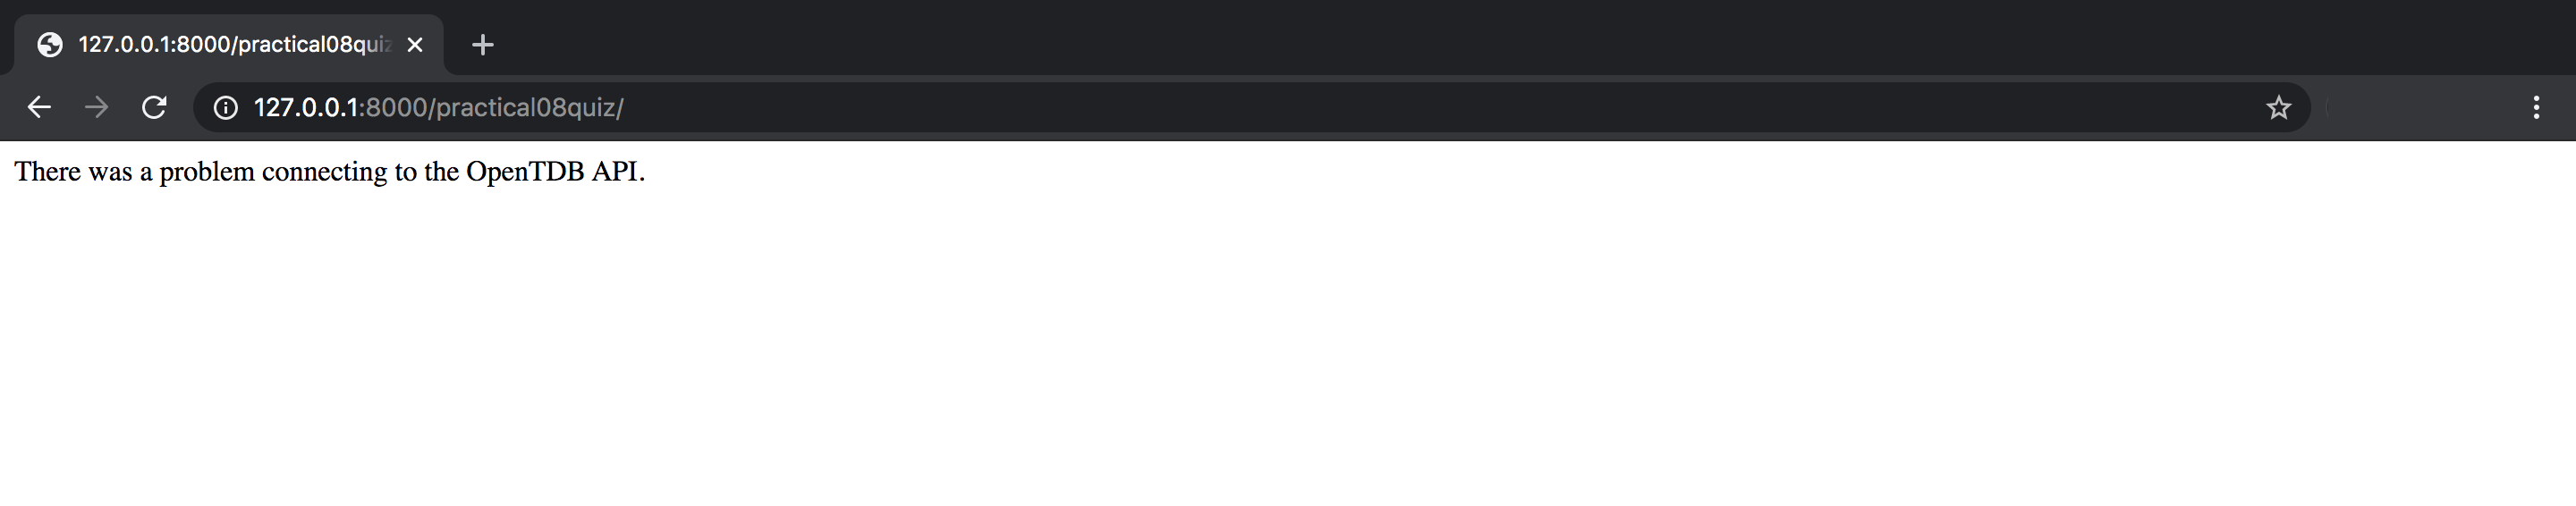
\includegraphics[width=175mm, height=35mm]{./img/08-expected-quiz-2.png}
\end{figure}

\textbf{Deployment link:} \href{https://int-app-dev-practical-08.herokuapp.com/practical08quiz/}{https://int-app-dev-practical-08.herokuapp.com/practical08quiz/} 

\subsection*{Resources} 
\begin{itemize}
  \item \href{https://opentdb.com/}{OpenTDB API}
  \item \href{https://requests.readthedocs.io/en/master/}{Requests}
  \item \href{https://requests.readthedocs.io/en/master/user/quickstart/\#json-response-content}{Requests JSON Response Content}
  \item \href{https://requests.readthedocs.io/en/master/api/#exceptions}{Requests Exceptions}
  \item \href{https://docs.djangoproject.com/en/3.0/ref/templates/builtins/#built-in-filter-reference}{Django Built-In Filters}
\end{itemize}

\section*{Task 2} 
Create a Django project called \texttt{dog}. \texttt{cd} to \texttt{dog}, create a virtual environment \& install Django. Create an app called \texttt{practical08dog}. Alternatively, you can create an app in \texttt{quiz}. Though, it requires additional configuration. Please ensure you configure your app in \texttt{dog/settings.py} \& \texttt{dog/urls.py}. \texttt{cd} to the \texttt{practical08dog} directory \& create a Python file called \texttt{urls.py}. In the \texttt{practical08dog} directory, create a directory called \texttt{templates} \& sub-directory called \texttt{practical08dog}. In \texttt{templates/practical08dog}, create a two \texttt{HTML} files called \texttt{index.html} \& \texttt{details.html}. \\

In \texttt{models.py}, create a class called \texttt{Dog} which extends \texttt{models.Model}. In \texttt{Dog}, declare the following: \\

\texttt{RANGE\_CHOICE = [('L', 'Low'), ('M', 'Medium'), ('H', 'High')]} \\

Above is a list containing tuples used as choices for a field. The first element in each tuple is the actual value to be set on the model \& the second element is the human-readable name. If choices are given to a field, they are enforced by model validation. The default form widget will be a select drop down containing choices as drop down options. \\

Below \texttt{RANGE\_CHOICE}, declare the following field names with their types \& options: 
\begin{verbatim}
  breed = models.CharField(max_length=200, unique=True) 
  height = models.IntegerField(default=1) 
  weight = models.IntegerField(default=1) 
  life_span = models.IntegerField(default=1) 
  adaptability = models.CharField(choices=RANGE_CHOICE, max_length=200) 
  friendliness = models.CharField(choices=RANGE_CHOICE, max_length=200) 
  grooming_needs = models.CharField(choices=RANGE_CHOICE, max_length=200) 
  trainability = models.CharField(choices=RANGE_CHOICE, max_length=200) 
  physical_needs = models.CharField(choices=RANGE_CHOICE, max_length=200) 
\end{verbatim}

For \texttt{Dog}, create a \texttt{\_\_str\_\_} method which returns \texttt{breed}. \\

In \texttt{views.py}, create two functions called \texttt{index} \& \texttt{details}. In the \texttt{index} function, render the \texttt{index.html} template with a \texttt{context} dictionary containing all \texttt{Dog} objects in the database. In \texttt{index.html}, display \texttt{context} in a nicely formatted \texttt{HTML} table. For \texttt{height}, \texttt{weight} \& \texttt{life\_span}, use the \texttt{pluralize} filter which returns a plural suffix if a value is not 1, '1' or an object of length 1. By default, this suffix is 's'. \texttt{height} will require an alternative suffix, i.e., 'es'. 

\begin{figure}[H]
  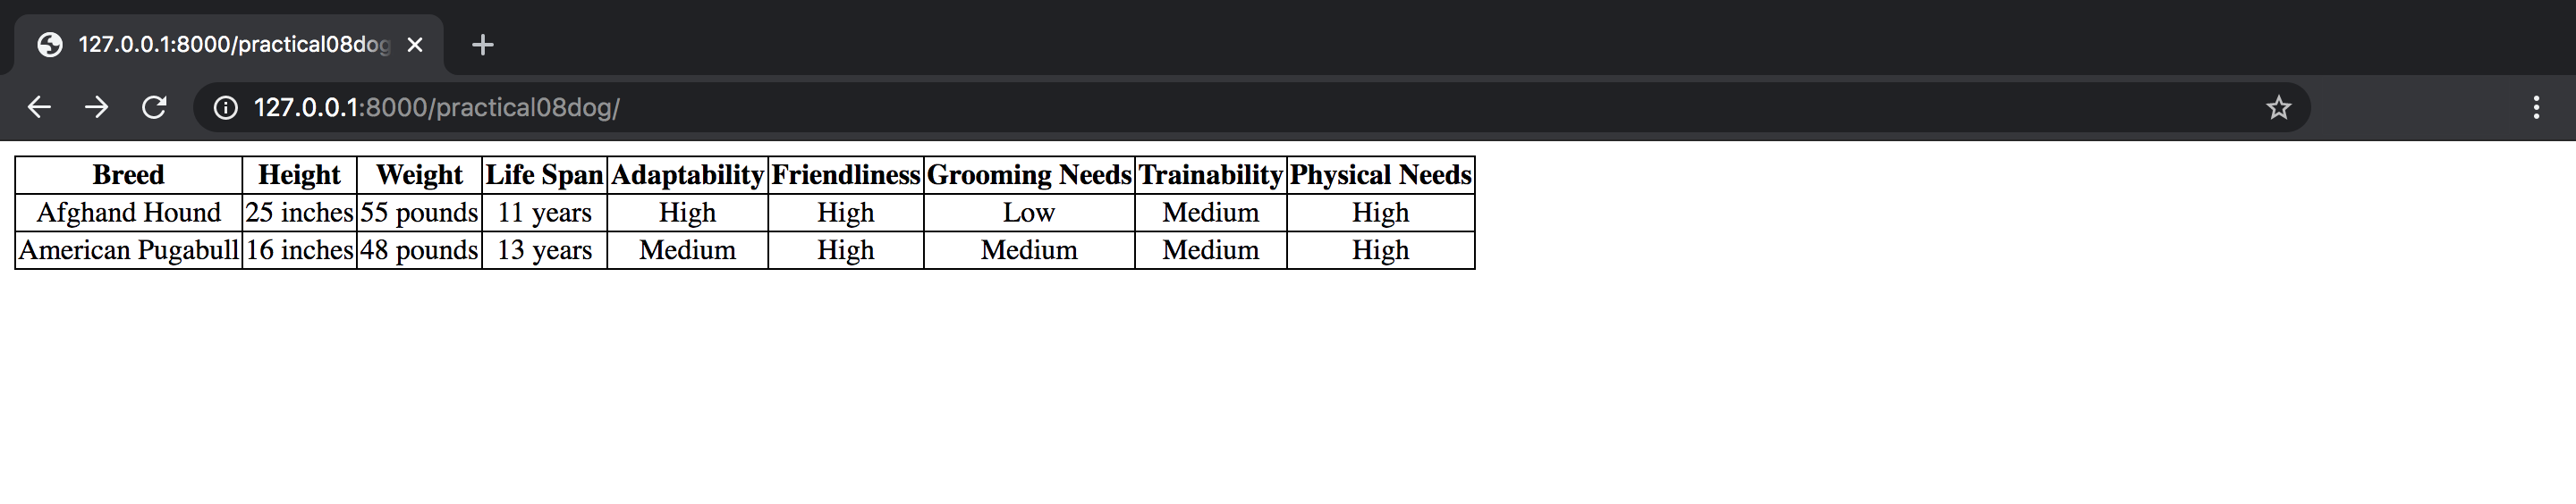
\includegraphics[width=175mm, height=35mm]{./img/08-expected-dog-1.png}
\end{figure}

In \texttt{index.html}, change each \texttt{breed} value to a link so when clicked, gets the \texttt{Dog} object by its id \& displays its details.

\begin{figure}[H]
  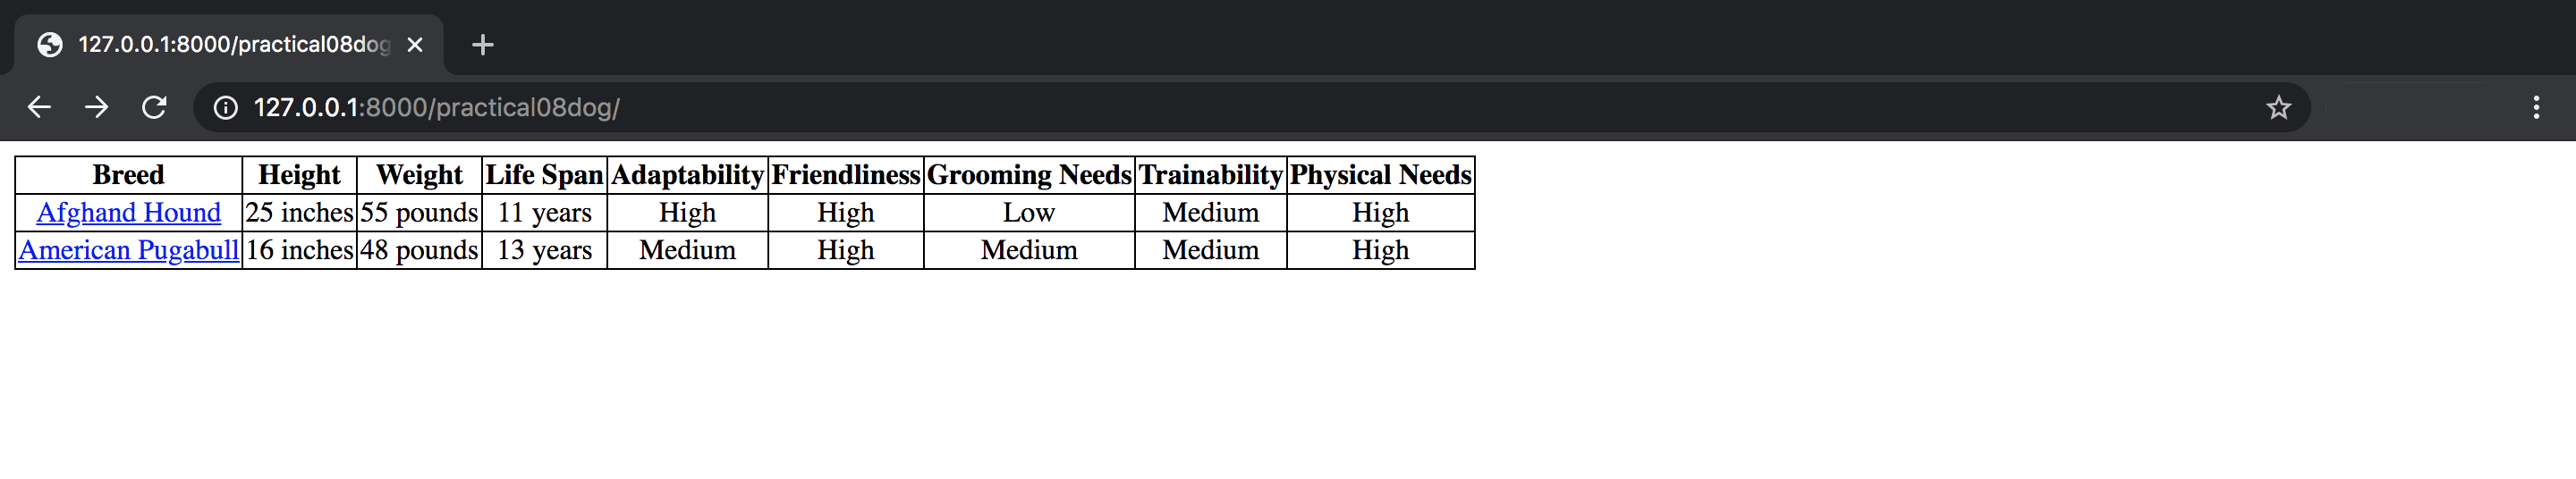
\includegraphics[width=175mm, height=35mm]{./img/08-expected-dog-2.png}
\end{figure} 

In the \texttt{details} function, render the \texttt{details.html} template with a \texttt{context} dictionary containing the \texttt{Dog} object with the primary key of, for example, 1 from \texttt{Dog}. Again, in \texttt{details.html}, display \texttt{context} in a nicely formatted \texttt{HTML} table \& use the \texttt{pluralize} filter for \texttt{height}, \texttt{weight} \& \texttt{life\_span}. 

\begin{figure}[H]
  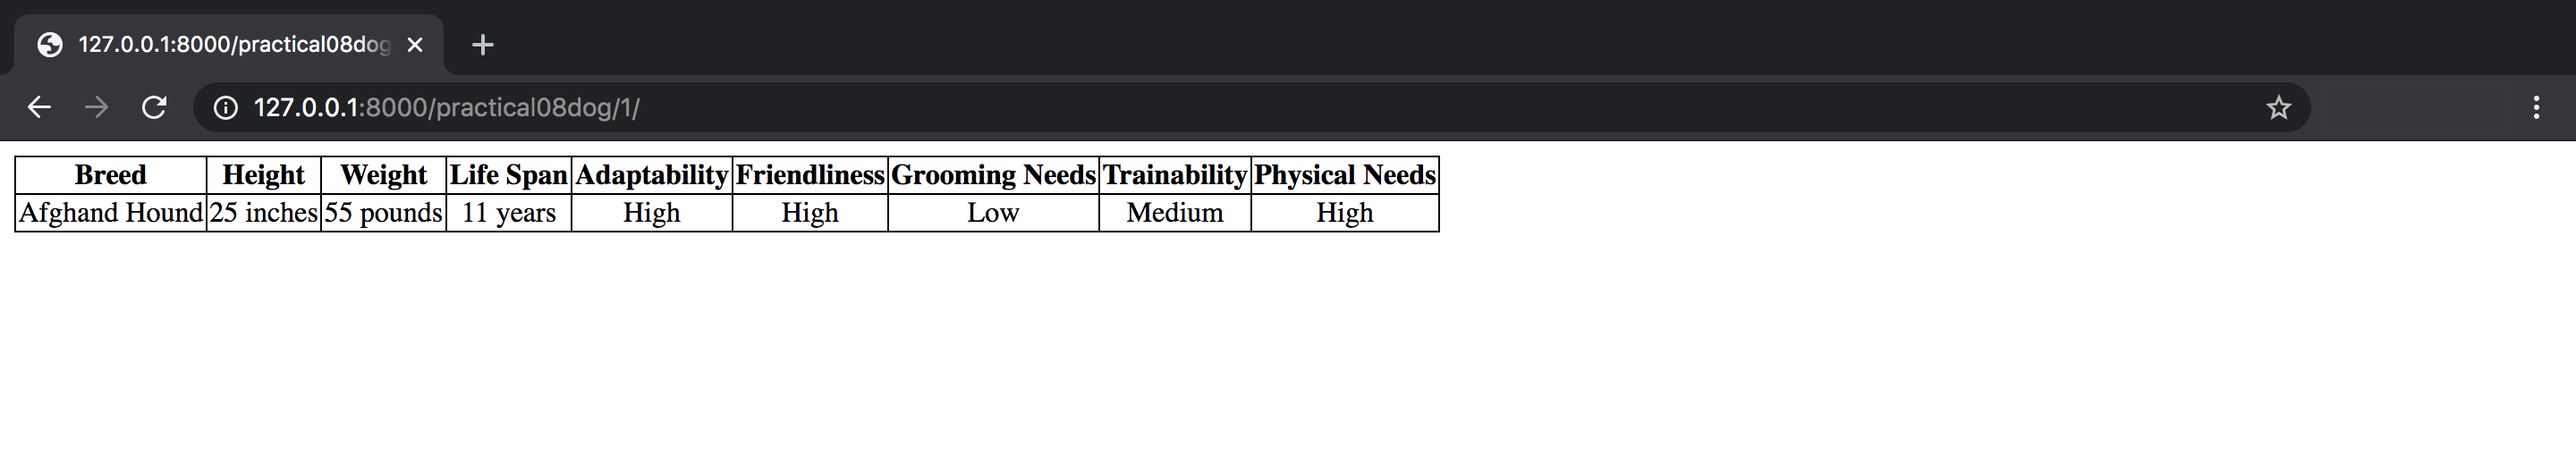
\includegraphics[width=175mm, height=35mm]{./img/08-expected-dog-3.png}
\end{figure}

In \texttt{urls.py}, set the \texttt{app\_name} to \texttt{practical08dog} \& create two URLs which map to the \texttt{index} \& \texttt{details} functions in \texttt{views.py}. 

\subsection*{Fixtures}  
In Django, you can pre-populate your database using migrations or fixtures. If you want to automatically load initial data, create a migration by running the command \texttt{python manage.py migrate}. Fixtures work slightly different as data is not automatically loaded like migrations. A fixture is a collection of data that Django knows how to import into a database. Fixtures can be written as \texttt{JSON}, \texttt{XML (Extensible Markup Language)} or \texttt{YAML (Yet Another Markup Language)}. Feel free to use any of the three formats. To start using fixtures, create a directory called \texttt{fixtures}. A \texttt{JSON} file called \texttt{dogs.json} has been provided for you in the \texttt{08-django-2-view-template} directory. Copy \& paste \texttt{dogs.json} into the \texttt{fixtures} directory. In \texttt{fixtures/dogs.json}, there are two \texttt{Dog} objects. Create two more \texttt{Dog} objects then run the command \texttt{python manage.py loaddata dogs.json}. You should see the following message in the terminal: \texttt{Installed 4 object(s) from 1 fixture(s)}.  \\

\subsection*{Expected Output} 
Run the command \texttt{python manage.py runserver} then navigate to \href{http://127.0.0.1:8000/practical08dog/}{http://127.0.0.1:8000/practical08dog/}

\begin{figure}[H]
  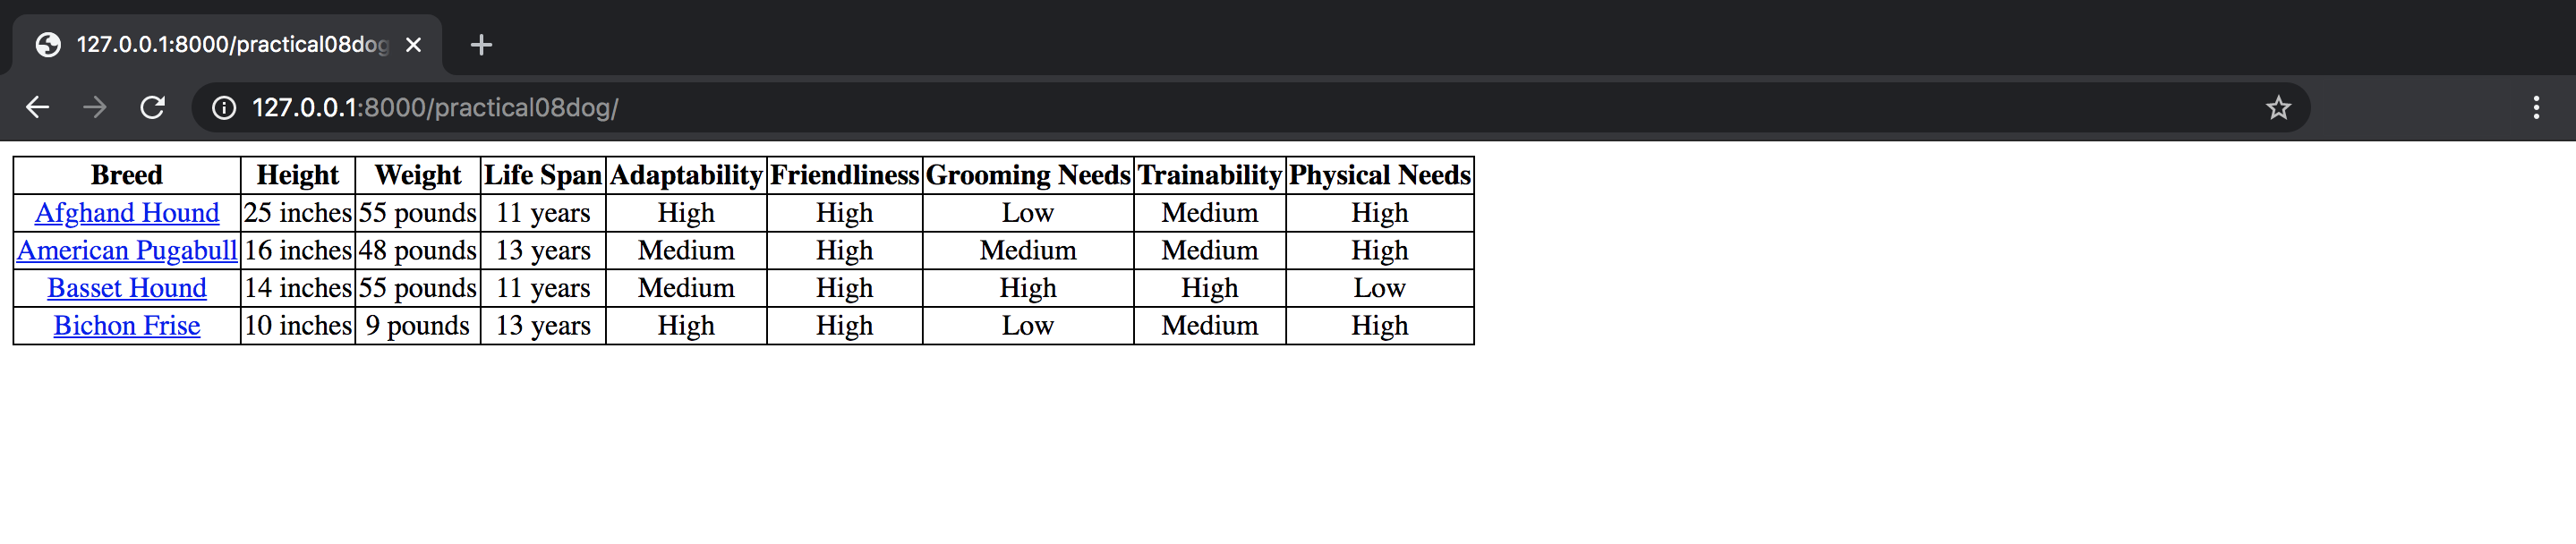
\includegraphics[width=175mm, height=35mm]{./img/08-expected-dog-4.png}
  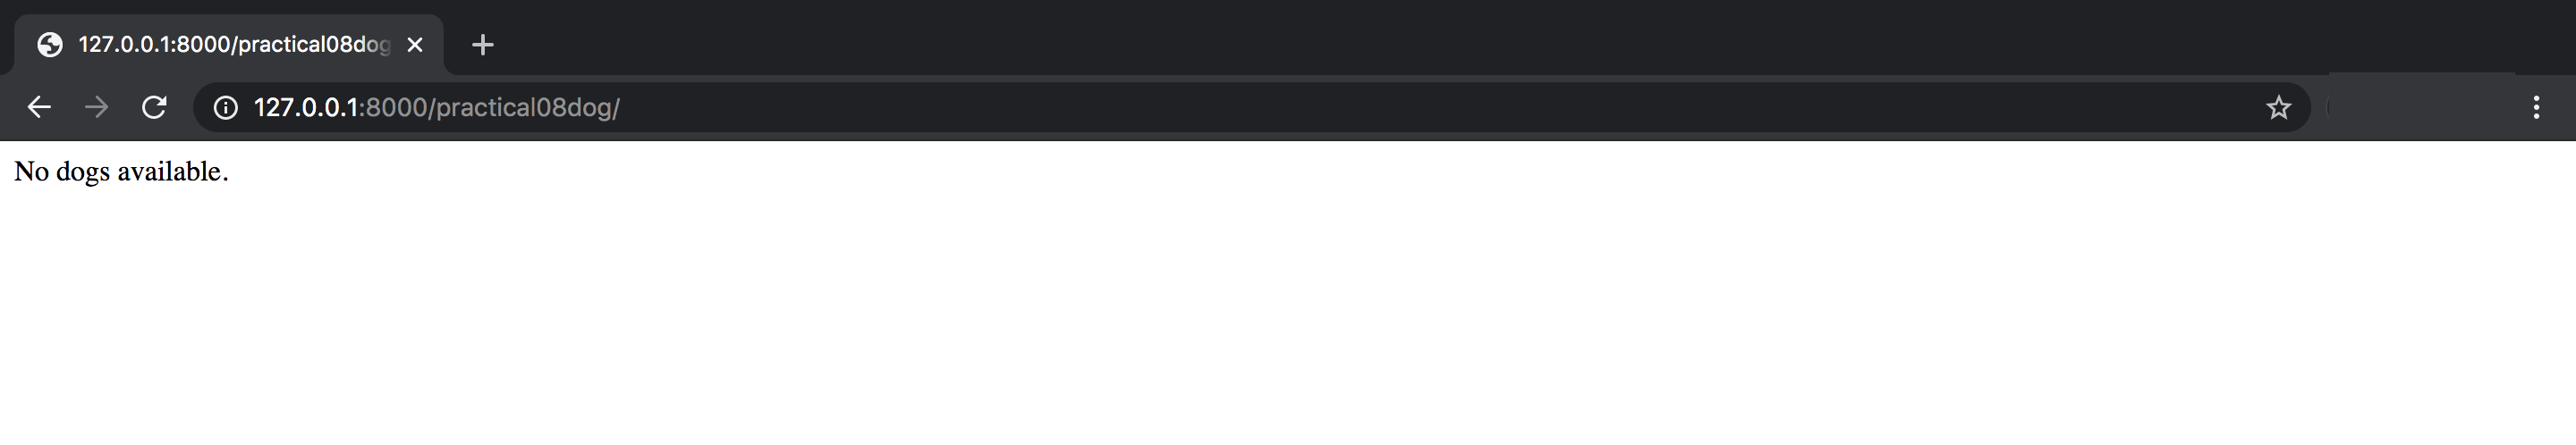
\includegraphics[width=175mm, height=35mm]{./img/08-expected-dog-5.png} 
\end{figure}

\textbf{Deployment link:} \href{https://int-app-dev-practical-08.herokuapp.com/practical08dog/}{https://int-app-dev-practical-08.herokuapp.com/practical08dog/}

\subsection*{Resources}
\begin{itemize}
  \item \href{https://docs.djangoproject.com/en/3.0/ref/models/fields/#module-django.db.models.fields}{Django Model Reference}
  \item \href{https://docs.djangoproject.com/en/3.0/ref/models/fields/#choices}{Django Choices}
  \item \href{https://docs.djangoproject.com/en/3.0/howto/initial-data/}{Django Fixtures}
\end{itemize}
 
\end{document}